\documentclass[12pt, fleqn]{article}
\usepackage{../../../template/template}
\usepackage{../../../template/fortickets}

%сам документ
\begin{document}
\begin{center}
  \huge Практика по матану, 3 сем

  \Large (преподаватель Роткевич А. С.)

  \large Записал Костин П.А.
\end{center}

Данный документ неидеальный, прошу сообщать о найденных недочетах в \href{https://vk.com/drab_existence_a}{вконтакте}
\tableofcontents
\newpage

%билеты
\section{Функции от нескольких переменных}
\subsection{02.09.2019}
\subsubsection{Основные определения}

\begin{definition}
    $\rho: X * X \ra \R$ - метрика, если
    \begin{enumerate}
    	\item $\rho(x,y) \geqslant 0$, $\rho(x,y)=0 \Lra x=y$
    	\item $\rho(x,y)=\rho(y,x)$
    	\item $\rho(x,y) \leqslant \rho(x,z)+\rho(z,y)$

    	$(X,\rho)$ - метрическое пространство
	\end{enumerate}
\end{definition}

\begin{examples}
    \begin{enumerate}
        \item $\R$ $\rho(x,y)=|x-y|$
        \item $x \neq \varnothing$ $\rho(x,y)=
            \begin{cases}
                1, \q x \neq y\\
                0, \q x=y
            \end{cases}$
        \item $\R^n$, $n \geqslant 1$ $\rho(x,y)=\sqrt{(x_1-y_1)^2+...+(x_n-y_n)^2}$,

        где $x=(x_1,...,x_n)$ $y=(y_1,...,y_n)$
    \end{enumerate}
\end{examples}

\begin{definition}
    $\rho_1, \rho_2: X*X \ra \R$ - метрики, тогда $\rho_1, \rho_2$ - эквивалентны, если

    (они задают одну топологию) $c_1 \rho_1 (x,y) \leqslant \rho_2 (x,y) \leqslant c_2 \rho_1(x,y)$ для $c_1,c_2>0$ - $\const$
\end{definition}

\begin{example}
    $\R^2$ $\rho_1(x,y) = \sqrt{(x_1-y_1)^2 + (x_2-y_2)^2} \leqslant \sqrt{2 \rho_2^2(x,y)}$

    $\rho_2(x,y)=max(|x_1-y_1|, |x_2-y_2|)$ (упр.)

    $\frac{1}{\sqrt{2}} \rho_1(x,y) \leqslant \rho_2(x,y) \leqslant \rho_1(x,y)$

    Пусть $\rho_3(x,y)=(|x_1-y_1|^p+...|x-n-y_n|^p)^{\frac{1}{p}}$, $p \geqslant 1$

    Если $p \ra \infty$ $\rho_3 \ra \rho_2$

    $l_n^p=(\R^n,\rho_3)$ - пространство Лебега конечномерное

    (упр.) Д-ть, что все метрики эквивалентны $(\rho_1,\rho_2,\rho_3)$

    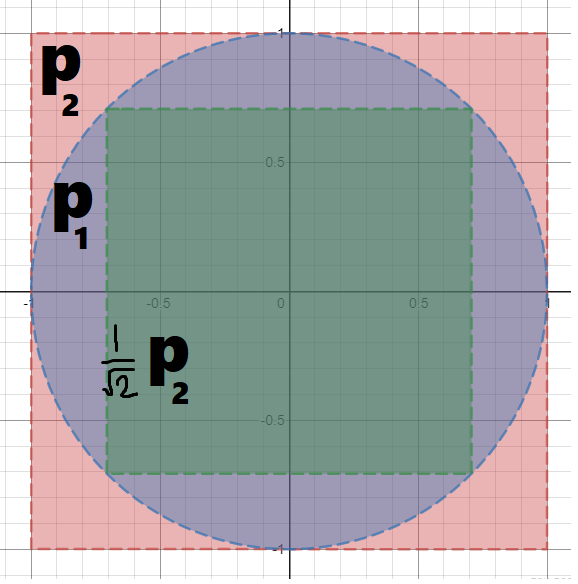
\includegraphics[scale=0.3]{pics/p1p2p3.png}
\end{example}

\begin{definition}
    $\rho: X*X \ra \R$ - метрика,

    Открытым шаром в X относительно метрики $\rho$ называется мн-во $B_r(x)=B(x,r)=\{y \in X: \rho(x,y) < r \}$

    Замкнутым шаром называется $\ol{B}_r(x)=\{y \in X: \rho(y,x) \leqslant r \}$

    Сферой называется $S_r(x)=\{y \in X: \rho(x,y)=r \}$
\end{definition}

\begin{upr}
    Замкнутый шар - не всегда замыкание шара (см. дискретную метрику)
\end{upr}

\begin{example}
    $l^p=\{ \{x_n\}_{n=1}^\infty: \sum\limits_{n=1}^\infty |x_n|^p < \infty \}$ $1 \leqslant p < \infty$

    $\rho(\{x_n\}_{n=1}^\infty, \{y_n\}_{n=1}^\infty) = (\sum\limits_{n=1}^\infty (x_n-y_n)^p)^{\frac{1}{p}}$

    $l^p$ - пр-во Лебега (последовательностей)
\end{example}

\begin{example}
    $C[0,1]$ - пр-во непр. функций

    $\rho(f,g)=\max\limits_{[0,1]} |f-g|$ - полна (любая фундаментальная последовательность сходится)

    $\rho_p(f,g)=(\int\limits_0^1 |f-g|^p dx)^{\frac{1}{p}}$ - не полная
\end{example}

\begin{definition}
    $(X, \rho)$ - метр. пр-во, $\{x_k\}_{k=1}^\infty \subset X$, $a \in X$ $x_k \ra a$ в пр-ве X по метрике $\rho$, если $\rho(x_n,a) \us{k \ra \infty}{\ra} 0$
\end{definition}

\begin{examples}
    $\R^2$ $M_k=(x_k, y_k)$ $P=(a,b)$ $M_k \ra P$ в евкл. метрике, т.е. $\rho(M_k,P)=\sqrt{(x_k-a)^2+(y_k-b)^2} \us{k \ra \infty}{\ra} 0 \Lra x_k \ra a,\ y_k \ra b$
\end{examples}

\begin{remark}
    Есть $\rho_1,\rho_2$ - экв. метрики, то $\rho_1(x_k,a) \ra 0 \Lra \rho_2(x_k,a) \ra 0$
\end{remark}

\begin{upr}
    $x_k \ra a,\ x_k \ra b \Ra a=b$

    ($\rho(a,b) \leqslant \rho(a, x_k) + \rho(x_k,b) \ra 0 \Ra \rho (a,b) \ra 0 \Ra a=b$)
\end{upr}

\begin{definition}
    $E \subset X$, $(X, \rho)$ - метр. пр-во, то $a \in X$ - т. сгущ. E, если

    $\forall \E \ \e x \in E: \rho(a,x) < \E$
\end{definition}

\begin{definition}
    $f:E \ra Y$ $(X, \rho)$, $(Y,d)$ - метр. пр-ва $(E \subset X)$, а - т. сгущ. E, $A \in Y$,

    тогда A - предел отображения f в точке а, если

    $f(x) \ra A$ при $x \in E \setminus \{a\}\ra a$\\
    (или $\forall \E>0 \q \e \delta>0: \rho(x,a)<\delta$ и $x \in E \subset \{a\}$, то $d(f(x),A) < \E)$\\
    Обозначение: $A=\lim\limits_{x \ra a} f(x)$ или $f(x) \ra A$ $x \ra a$
\end{definition}

\begin{remark}
    $A=\lim\limits_{x \ra a} f(x) \Lra \forall \E > 0 \ \e \delta>0: f(B_\delta(a) \setminus \{a\}) \subset B_\E (A)$
\end{remark}

\newpage
\subsection{05.09.2019}
\subsubsection{Примеры для $\R^2$}

Будем в $\R^2$, $\rho((x_1,y_1), (x_2,y_2)) = \sqrt{(x_1-x_2)^2 + (y_1-y_2)^2}$
\begin{definition}
    $f: E \ra \R$, $E \subset \R^2$, $a \in \R^2$ - точка сгущения, $\lim\limits_{x \ra a} f(x) = F$, если

    $\forall \E>0 \q \e \delta>0: 0<\rho(x,a)<\delta$, $x \in E \Ra |f(x)-A|<\E$
\end{definition}
В $\R^2$ работают:

арифм. действия, теор. о двух миллиционерах, критерий Коши:
\begin{definition}
    $f: E \ra \R$, частный случай $\e \lim\limits_{x \ra a} f \Lra \forall \E>0 \q \e \delta > 0:$

    $|f(x)-f(y)|<\E$ $0<\rho(x,a), \rho(y,a)<\delta$ (упр)
\end{definition}

\begin{upr}
    $\e \lim\limits_{x \ra a} f \Lra \forall \{x_n\}: x_n \neq a \q x_n \ra a$ ($\rho(x_n,a) \ra 0$) $\e \lim\limits_{n \ra \infty} f(x_n)$
\end{upr}

Обозначение: $\us{y \ra y_0}{\lim\limits_{x \ra x_0}} f(x,y) = \lim\limits_{(x,y) \ra (x_0,y_0)} f(x,y)$ - предел функции в т. $(x_0,y_0)$

\begin{example}
    $f(x,y)=(x+y)\sin \frac{1}{x} \sin \frac{1}{y}$, $\us{y \ra 0}{\lim\limits_{x \ra 0}} f(x,y) = 0$, т.к.$|f(x,y)| \leqslant |x|+|y| \us{y \ra 0}{\us{x \ra 0}{\ra}} 0$, $\not \e \lim\limits_{y \ra 0} \lim\limits_{x \ra y} f(x,y)$
\end{example}

\begin{example}\\
    $f(x,y)=\frac{x^2 y^2}{x^2 y^2 + (x-y)^2}$ - не существует, так как $\lim f(x,x)=1$, $f(x,2x)=0$
\end{example}

\begin{example}
    Построить $f(x,y)$ т.ч. $\forall a,b$ $\e \lim\limits_{t \ra 0} f(at,bt)=A$, но $\not \e \us{y \ra 0}{\lim\limits_{x \ra 0}} f(x,y)$

    $f=\frac{y^2}{x}=\frac{b^2}{a} t \ra 0$, но при $x=\frac{1}{n^2}$, $y=\frac{1}{n}$ предел - единица
\end{example}

\begin{remark}
    Если $\upgamma(t) \us{t \ra t_0}{a} \in \R^2$ и $\e \lim\limits_{x \ra a} f(x)=A$, то $\e \lim\limits_{t \ra t_0} f(\upgamma(t))$
\end{remark}

\begin{remark}
    Если $\forall \upgamma: \upgamma(t) \ra a \in \R^2$ и $\e \lim f(\upgamma(t))$, то $\e \lim\limits_{x \ra a} f$
\end{remark}

\begin{remark}
    $\lim\limits_{x \ra x_0} \lim\limits_{y \ra y_0} f(x,y)$ - не предел по кривой (из-за необязательного равенства предела и значения в пределе). Более формально: пусть $=\lim\limits_{x \ra x_0} \ol{f}(x)$

    $\ol{f}(x)=\lim\limits_{y \ra y_0} f(x,y) \neq$(не обязательно) $\neq f(x,y_0)$
\end{remark}

\begin{definition}\\
    $\us{y \ra +\infty}{\lim\limits_{x \ra +\infty}} f(x,y)=A$, если

    $\forall \E>0 \ \e M>0: \forall x,y: \max(x,y)>M \ |f(x,y)-A|<\E$
\end{definition}

\begin{example}\\
    $f=\frac{y}{x} tg(\frac{x}{x+y})$ - не имеет предела, $f(x,x)=tg(\frac{1}{2})$, $f(x,x^2)=x tg(\frac{1}{1+x}) \ra 0$
\end{example}

\newpage
\subsection{09.09.2019}
\subsubsection{Ещё больше определений}
\begin{definition}
\begin{enumerate}
        \item $A=\us{y \ra +\infty}{\lim\limits_{x \ra +\infty}} f(x,y)$, если

        $\forall \E>0 \ \e M>0: x>M \ y>M \Ra |f(x,y)-A| < \E$
        \item $A=\us{y \ra +\infty}{\lim\limits_{x \ra +\infty}} f(x,y)$, если

        $\forall \E>0 \ \e M>0: |x|>M \ |y|>M \Ra |f(x,y)-A| < \E$
        \item $A=\lim\limits_{P \ra \infty} f(P) \ P \in \R^2$, если

        $\forall \E>0 \ \e M>0: \rho(0, P)>M \Ra |f(x,y)-A| < \E$
    \end{enumerate}
\end{definition}

\begin{remark}
    Демидович по первым двум определениям
\end{remark}

\begin{definition}
    Для конечного предела: $A=\lim\limits_{x \ra a \  y \ra +\infty} f(x,y)$, если

    $\forall \E>0 \q \e M>0 \q \delta > 0: y>M \q |x-a| < \delta \Ra |f(x,y)-A| < \E$
\end{definition}

\subsubsection{Ещё больше примеров}

\begin{example}
    $\us{y \ra +\infty}{\lim\limits_{x \ra +\infty}} (\dfrac{x y}{x^2+y^2})^{x^2}$
\end{example}

\begin{sol}
    Заметим, что $\dfrac{x y}{x^2+y^2} \leqslant \dfrac{1}{2} \Ra 2xy \leqslant x^2 + y^2 \Ra 0 \leqslant (x-y)^2\text{ для x }\neq y$
    \\
    Значит дробь стремится к 0
\end{sol}

\begin{example}
    $\us{y \ra 0}{\lim\limits_{x \ra 0}} (\dfrac{x y}{x^2+y^2})^{x^2}$
\end{example}

\begin{sol}
    При $x=y$ предел $\dfrac{1}{2}$\\
    При $x=y^2$ предел 0
\end{sol}

\begin{example}
    $f=\sin(\dfrac{\pi y^2}{x^2 + 3y^2})$\\
    Найти $\us{y \ra +\infty}{\lim\limits_{x \ra +\infty}} f$, $\lim\limits_{x \ra \infty} \lim\limits_{y \ra \infty} f$, $\lim\limits_{y \ra \infty} \lim\limits_{x \ra \infty} f$
\end{example}

\begin{sol}
    Первый не имеет предела ($x=y$, $x=\sqrt{y})$. Второй $\dfrac{\sqrt{3}}{2}$. Третий 0
\end{sol}

\begin{example}
    $\us{y \ra +\infty}{\lim\limits_{x \ra +\infty}} \dfrac{sin(y-x^2)}{y-x^2}$
\end{example}

\begin{sol}
    $z=y-x^2$, $z \ra 0 \Ra x,y \ra 0$

    $|z| \leqslant |x| + |y| \leqslant 2 \sqrt{x^2+y^2}$
\end{sol}

\begin{example}
    $f=\dfrac{1-\sqrt[3]{sin^4 x + cos^4 y}}{\sqrt{x^2+y^2}}$, найти $\us{y \ra 0}{\lim\limits_{x \ra 0}} f$
\end{example}

\begin{sol}
    $1-\sqrt[3]{t} \us{t \ra 1}{~} \dfrac{1-t}{3}$ (т.к. $1-\sqrt[3]{t}=\frac{1-t}{1+\sqrt[5]{t}+\sqrt[3]{t^2}}$)

    Значит $\us{y \ra 0}{\lim\limits_{x \ra 0}} f = \us{y \ra 0}{\lim\limits_{x \ra 0}} \frac{1}{3} \dfrac{1-(sin^4 x + cos^4 y)}{\sqrt{x^2+y^2}} = \us{y \ra 0}{\lim\limits_{x \ra 0}} \dfrac{2sin^2 y - sin^4 y - sin^4 x}{3 \sqrt{x^2+y^2}}$

    Заменим по Тейлору: $=\us{y \ra 0}{\lim\limits_{x \ra 0}} \dfrac{2y^2 + \ol{o}(y^3)-x^4 + \ol{o}(x^6)}{3 \sqrt{x^2+y^2}}$

    Попробуем оценить по модулю $|\dfrac{2y^2-x^4}{\sqrt{x^2+y^2}}|$, заметим что $y^2 \leqslant x^2 + y^2$,

    $x^4 \leqslant 2(x^2+y^2) \leqslant x^2+y^2$ (для $x^2+y^2 < 1)$,

    чтобы избавиться от $\ol{o}$ оценим так:

    $\ol{o} + y^2 \leqslant 2(x^2 + y^2)$, $\ol{o} + x^4 \leqslant 2(x^2+y^2) \leqslant x^2+y^2$

    Тогда $|\dfrac{2y^2-x^4}{\sqrt{x^2+y^2}}| \leqslant 2 \dfrac{3(x^2+y^2)}{\sqrt{x^2+y^2}} \leqslant 6 \sqrt{x^2+y^2} \ra 0$
\end{sol}

\newpage
\subsection{12.09.2019}
\subsubsection{Некоторые особенные примеры}
\begin{example}
    $\us{y \ra 1}{\lim\limits_{x \ra 0}} (1+x)^{\frac{1}{x+x^2 y}}=\us{y \ra 1}{\lim\limits_{x \ra 0}} ((1+x)^{\frac{1}{x}})^{\frac{1}{1+x y}}=e$
\end{example}

\begin{example}
    $f(x,y)=\begin{cases} \frac{x^3-xy^2}{x^2+y^2} &,x^2+2^2 \neq 0\\ a & , else \end{cases}$\\
    1) $a=?$, т.ч. f - непр\\
    2) $a=?$, f - непрю на прямых, проходящих через 0\\
\end{example}

\begin{sol}
    1) $a=\us{y \ra 0}{\lim\limits_{x \ra 0}} \frac{x^3-x y^2}{x^2+y^2}=\us{y \ra 0}{\lim\limits_{x \ra 0}} x \frac{x^2-y^2}{x^2+y^2}=0$
\end{sol}

\begin{remark}
    $x^n y^m \leqslant (\sqrt{x^2+y^2})^{n+m}$ и $|x| \leqslant \sqrt{x^2+y^2}$
\end{remark}

\subsubsection{Частные производные. Определения}
$f: \Omega \subset \R^3 \ra \R$, $P_0=(x_0,y_0,z_0)$
\begin{definition}
    f - диф. в точке $P_0$, если $\e A,B,C \in \R$, т.ч.\\
    $f(x_0,+\delta x, y_0 + \delta y, z+\delta z =f(x_0,y_0,z_0)+A \delta x+ B \delta y + C \delta z+\ol{o} (\sqrt{(\delta x)^2+(\delta y)^2+ (\delta z)^2})$\\
    Пусть $h=(\delta x, \delta y, \delta z)^T$\\
    $f(P_0+h)=f(P_0)=\begin{pmatrix} A\\ B\\ C \end{pmatrix}^T h + \ol{o}(|h|)$\\
    $df(x,y,z)=A dx+B dy+C dz$\\
    Дифференциал сопоставляет $(dx, dy, dz) \ra A dx+B dy+C dz$
\end{definition}

\begin{definition}
    Частной произв. по перем. x в т. $(x_0,y_0,z_0)$ называется предел (если $\e$)
    \[\lim\limits_{t \ra 0} \frac{f(x_0+t,y_0,t_0)-f(x_0,y_0,z_0)}{t}=\frac{\d f}{\d x}(x_0,y_0,z_0)=f'_x(x_0,y_0,z_0)\]
\end{definition}

\subsubsection{Частные производные. Примеры}
\begin{utv}
    f - дифф. $\Ra$ $\e$ част. пр. и $A= \frac{\d f}{\d x} (x_0,y_0,z_0)$, $B=\frac{\d f}{\d x}$, $C=\frac{\d f}{\d x}$
\end{utv}

Производные старшего порядка \[\frac{\d^2 f}{\d x^2} = \frac{\d}{\d x} (\frac{\d f}{\d x})\]
\[\frac{\d^2 f}{\d x \d y}= \frac{\d}{\d x} \frac{\d f}{\d y} \neq \text{(не всегда) }\frac{\d}{\d y} (\frac{\d f}{\d x}) = \frac{\d^2 f}{\d y \d x}\]

Частные производные сложной функции
\[w=f(x,y,z),\ \R^2 \ra \R^3.\ (u,v) \ra(\varphi(u,v), \psi(u,v), \chi(u,v))\]
\[w=f(\varphi(u,v), \psi(u,v), \chi(u,v))\]
\[\frac{\d w}{\d u}=\frac{\d f}{\d x}, \frac{\d \varphi}{\d u}+ \frac{\d f}{\d y} \frac{\d \psi}{\d u}+\frac{\d f}{\d z} \frac{\d \chi}{\d u}\]
\[\frac{\d w}{\d v}=\frac{\d f}{\d x} \frac{\d \varphi}{\d v}+\frac{\d f}{\d y} \frac{\d \psi}{\d v}+ \frac{\d f}{\d z} \frac{\d \chi}{\d v}\]
\[
\begin{pmatrix}
\dfrac{\d w}{\d u}\\
\dfrac{\d w}{\d v}
\end{pmatrix}=
\begin{pmatrix}
\dfrac{\d \varphi}{\d u} & \dfrac{\d \psi}{\d u} & \dfrac{\d \chi}{\d u}\\
\dfrac{\d \varphi}{\d v} & \dfrac{\d \psi}{\d v} & \dfrac{\d \chi}{\d v}
\end{pmatrix}
\begin{pmatrix}
\dfrac{\d f}{\d x}\\
\dfrac{\d f}{\d y}\\
\dfrac{\d f}{\d z}
\end{pmatrix}
\]

\begin{Example}
    \[\frac{\d^2 w}{\d u \d v} = \frac{\d f}{\d x} \frac{\d^2 \varphi}{\d u \d v}+(\frac{\d^2 f}{\d x^2} \frac{\d u}{\d v}+\frac{\d^2 f}{\d x \d y} \frac{\d \psi}{\d v}+\frac{\d^2 f}{\d x \d z} \frac{\d \chi}{\d v}) \frac{\d \varphi}{\d u}+...\]
\end{Example}

\begin{Example}
    \[F=f(x,x y, x y z)=f(u,v,w)\]
    \[\frac{\d F}{\d x}=\frac{\d f}{\d u} 1+ \frac{\d f}{\d v} y + \frac{\d f}{\d w} yz\]
    \[\frac{\d}{\d x}=\frac{\d}{\d u}+y \frac{\d}{\d v}+uz \frac{\d}{\d w}\]
    \[\frac{\d^2 F}{\d x^2} = \frac{\d}{\d x}(\frac{\d f}{\d u})+ \frac{\d}{\d x}(\frac{\d f}{\d v}) y + \us{=0}{\frac{\d f}{\d v} \frac{\d}{\d x} (y)}+ \frac{\d}{\d x} (\frac{\d f}{\d w}) yz + \frac{\d f}{\d w} \frac{\d}{\d x} (yz)\]
    \begin{multline*}
        \frac{\d}{\d x} (\frac{\d f}{\d u})=\frac{\d^2 f}{\d u^2}+ y \frac{\d^2 f}{\d u \d v}+yz \frac{\d^2 f}{\d u \d w} =\\ = \frac{\d^2 f}{\d u^2}+y \frac{\d^2 f}{\d v^2}+(yz)^2 \frac{\d^2 f}{\d w^2}+z y \frac{\d^2 f}{\d u \d v} + 2y^2 z \frac{\d^2 f}{\d v \d w} + 2yz \frac{\d^2 f}{\d u \d w}
    \end{multline*}
\end{Example}

\begin{example}
    Дано $u=x^y$, найти $\dfrac{\d^2 u}{\d x^2}$, $\dfrac{\d^2 u}{\d y^2}$, $\dfrac{\d^2 u}{\d x \d y}$
    \\
    \[\dfrac{\d u}{\d x}=y x^{y-1}, \q \dfrac{d^2 u}{\d x^2}=y(y-1)x^{y-2}\]
    \[\dfrac{\d u}{\d y}=\ln(x) x^y, \q \dfrac{\d^2 y}{\d y^2}=\ln^2(x) x^y\]
    \[\dfrac{\d^2 u}{\d x \d y}=x^{y-1}+y \ln(x) x^{y-1}\]
\end{example}

\newpage
\subsection{16.09.2019}
\begin{example}
    Выяснить, есть ли производная у $f(x,y)=\sqrt[3]{x^3+y^3}$
\end{example}

\begin{Sol}
    \[\dfrac{\d f}{\d x}=\dfrac{x^2}{\sqrt[3]{(x^3+y^3)^2}},\q x^3+y^3 \neq 0\]
    \[\dfrac{\d f}{\d x}(0,0)=\lim\limits_{t \ra 0} \dfrac{\sqrt[3]{t^3+0^3}-\sqrt[3]{o^3+0^3}}{t}=1\]
    \[\us{y \ra 0}{\lim\limits_{x \ra 0}}\text{ не }\e\]

    Пусть $\sqrt[3]{x^3+y^3}$ - диф. в точке $(0,0)$ $\Ra$
    \[\sqrt[3]{x^3+y^3}=0+x+y+\ol{o}(\sqrt{x^2+y^2})\]
    \[\sqrt[3]{(0+\delta x)^3+(0+\delta y)^3}=\us{=0}{f(x,y)}+\us{=1}{\dfrac{\d f}{\d x}(0,0) \delta x}+\us{=1}{\dfrac{\d f}{\d x}(0,0) \delta y}+\ol{o}(\sqrt{\delta x^2+\delta y^2})\]
    \[\sqrt[3]{x^3+y^3} = x+y+\ol{o}(\sqrt{x^2+y^2}),\q x,y \ra 0\]
    \[x_n=y_n \q \sqrt[3]{2}x=2x+\ol{o}(x)\]
    \[\sqrt[3]{2}-2=\ol{o}(1) ?!!\]
    То есть из существования ч.п. не следует дифференцируемость
\end{Sol}

\begin{theorem}
    Если существуют ч.п. и они непр. в рассм. точке $\Ra$ ф-ия диф. в этой точке
\end{theorem}

\begin{example}
    $f(x,y)=xy \dfrac{x^2-y^2}{x^2+y^2}$, $f(0,0)=0$ $\Ra$ f - непр. в 0
    \[g(x,y)=\frac{\d f}{\d x}= \dfrac{3 x^2 y-y^3}{x^2+y^2}-2x^2 y \dfrac{x^2-y^2}{(x^2+y^2)}, \q \frac{\d f}{\d x}(0,0)=0 \]
    \[\frac{\d}{\d y}(\dfrac{\d f}{\d x}) |_{(0,0)}=\lim\limits_{t \ra 0}(\dfrac{-\dfrac{t^3}{t^2}-0}{t})=-1\]
    Аналогично $\dfrac{\d f}{\d x}=0$, $\dfrac{\d}{\d x}(\dfrac{\d f}{\d y})=1$
\end{example}

\begin{theorem}
    Если $\dfrac{\d^2 f}{\d x \d y}$ и $\dfrac{\d^2 f}{\d y \d x}$ $\e$ в окр. точки, непр. в этой точке $\Ra$ в этой точке $\dfrac{\d^2 f}{\d x \d y} = \dfrac{\d^2 f}{\d y \d x}$
\end{theorem}

\subsubsection{Дифференцирование неявных функций}
\begin{definition}
    $F: \R^n \times \R \ra \R$ $F(x_1,...,x_n;y)$, $F(x_1^0,...,x_n^0;y^0)=0$

    $y=f(x_1,...,x_n)$ - ф-ия задана неявно уравнением $F(x_1,...,x_n;y)=0$ в откр. точке $(x_1^0,...,x_n^0, y^0)$, если ($x=(x_1,...,x_n)$):
    \begin{enumerate}
        \item $\us=F(x,f(x))=0$ (в окр. $x^0$)
        \item $f(x^0)=y^0$
    \end{enumerate}
\end{definition}

\begin{Theorem}[о неявном отображении]
    \[F: \R^n \times \R \ra \R,\q F(x^0,y^0)=0,\text{ F - непр. диф. в окр } (x^0,y^0),\]
    \[F'_y(x^0,y^0) \neq 0, \text{ тогда:}\]
    \begin{enumerate}
        \item $\e y=f(x_1,...,x_n)$ зад. неявно ур. $F(x,y)=0$
        \item f диф. в окр. $x^0$
        \item $\dfrac{\d f}{\d x_0}=-\dfrac{\d F}{\d x_0}/\dfrac{\d F}{\d y}$ в окр. $x^0$
    \end{enumerate}
\end{Theorem}

\newpage
\subsection{19.09.2019}
\subsubsection{Неявные функции наносят ответный удар}

\begin{Example}
    \[F(x,y)=y e^y+x+x^2=0\]
    \[y(x)=y(0)+y'(0)x+\frac{y''(0)}{2}x^2+...+\frac{g^{(n)}(0)}{n!}x^n+\ol{o}(x^n), \text{ при } x \ra 0\]
    \[x_0=0 \q y(0)=? \q y e^y=0 \q y=0\]
    \[F'y=e^y+y e^y |_{(0,0)} = 1 \neq 0\]
    \[y'(0)=-\frac{F'_x}{F'_y}|_{(0,0)}=-\frac{1+2x}{1}=-1 \text{ т.о. неявное отображение}\]
    \[y'(x)=-\frac{F'_x}{F'_y}=-\dfrac{1+2x}{(y(x)+1)e^{y(x)}}\]
    \[y(x)=0-x+\ol{o}(x)\]
    Что теперь делать? Способ 1:
    \[y''(x)=(y'(x))'=(-\frac{F'_x(x,y(x))}{F'_y(x,y(x))})'=(-\frac{1+2x}{(y(x)+1)e^{y(x)}})'\]
    \[=-\frac{2}{(y(x)+1)e^{y(x)}}+\frac{1+2x}{((y(x)+1)e^{y(x)}}(y(x)+2)e^{y(x)}y'(x) \us{\us{\large y=0}{x=0}}{=}-2-4=-6\]
    Наш ряд Тэйлора:
    \[y(x)=-x-3x^2+\ol{o}(x^2)\]
    Способ 2 (метод неопр. коэффициентов)
    \[y(x)=-x+a x^2+b x^3+\ol{o}(x^3)\]
    \[F(x,y(x))=0 \text{ в опр x=0}\]
    \[(-x+a x^2+b x^3+\ol{o}(x^3)) e^{-x+a x^2+b x^3+\ol{o}(x^3)}+x+x^2=0\]
    \[e^t=1+t+\frac{t^2}{2}+\frac{t^3}{6}+\ol{o}(t^3),\q t \ra 0\]
    \[t=y(x)\]
    \begin{multline*}
        (-x+a x^2+b x^3)[1+(-x+a x^2+b x^3)+\frac{(-x+a x^2+b x^3)^2}{2}+\\+\frac{(-x+a x^2+ b x^3)^3}{6}+o(x^2)]+x+x^2=0
    \end{multline*}
    \[F(x,y)=y e^y+x+x^2=0\]
    \[(-x+a x^2+b x^3+\ol{o}(x^3))(1-x+(a+\frac{1}{2})x^2+(b-a-\frac{1}{6})x^3+\ol{o}(x^3))+x+x^2=0\]
    \[\ol{o}(x^3)-x+x^2(1+a)+x^3 (b-a-a-\frac{1}{2})+x+x^2=0\]
    \[\ol{o}(x^3)+(a+2)x2+(b-2a-\frac{1}{2})x^3=0\]
    \[\begin{cases} a+2=0\\ b-2a-\frac{1}{2}=0 \end{cases} \text{ система должна быть диагональной}\]
    \[a=-2 \q b=-\frac{7}{2}\]
\end{Example}

\begin{Example}
    \[\cos(x y)+\sin x+e^{y+x}=2\]
    Проверить условие т.о неявной ф-ии и найти разл y(x) по Тейллору до $\ol{o}(x^3)$
    \[x=0, \q F(0,y)=0 \ra y(0)\]
    \begin{enumerate}
        \item $1+e^y=2$, $y=0$, $F(0,0)=0$, $y(0)=0$
        \item $F'_y=-x \sin(xy)+e^{y+x}|_{(0,0)}=1 \neq 0$\\
        $F'_x=-y \sin(xy)+\cos(x)+e^{y+x}|_{(0,0)}=2$\\
        $y'(0)=-2$
    \end{enumerate}
    Методом неявных коэффициентов
    \[y(x)=-2x+ax^2+b x^3+\ol{o}(x^3)\]
    \[\cos(-2x^2+a x^3+b x^4+\ol{o}(x^4))+\sin x+e^{-x+a x^2 + b x^3+\ol{o}(x^3)}=...\]
\end{Example}

\newpage
\subsection{23.09.2019}

\[F(u;x,y)=0\]
\[\left.
  \begin{array}{ccc}
     F(u_0;x_0,y_0) & = & 0\\
     F'_u(u_0;x_0,y_0) & \neq & 0
  \end{array}
\right.
\Ra
\left.
  \begin{array}{ccc}
    \text{$\e$ неявная ф-ия $u(x,y)$}\\
     u(x_0,y_0)=u_0 \\
     F(u(x,y),x,y)=0 \\
     u'_x=-\dfrac{F'_x}{F'_u}\\
     u'_y=-\dfrac{F'_y}{F'_u}
  \end{array}
\right.
\]
Ф-ла Тейлора для функцийи от неск. перем.
\[u: E \subset \R^n \ra \R, \q x \in E \ra u(x)\]
\[T_R(x,x^0)=\sum_{|\alpha| \leqslant k} \dfrac{\d^{\alpha} u(x^0)}{\d x^{\alpha}} \dfrac{(x-x^0)^{\alpha}}{\alpha!}=\sum_{j=0}^k \dfrac{d^j u(x^0) [x-x^0]}{j!}\]
\[\alpha\text{ - мультииндекс}, \q \alpha=(\alpha_1,...,\alpha_k), \q \alpha_j \in \N \cup \{0\}\]
\[|\alpha|=\alpha_1+...+\alpha_n, \q \alpha!=\alpha_1!...\alpha_n!\]
\[\dfrac{\d^{\alpha} u}{\d x^{\alpha}}=\dfrac{\d^{|\alpha|}}{\d x_1^{\alpha_1}...x_n^{\alpha_n}}, \q (x-x_0)^{\alpha} = (x_1-x_1^0)^{\alpha_1}...(x_n-x_n^0)^{\alpha_n}\]

\begin{Theorem}
    \[u \in C^k \os{\text{в окр. $x^0$}}{\Ra} \]
\end{Theorem}
\begin{Example}
    \[u: \R^2 \ra \R\]
    \begin{multline*}
        $$u(x,y)=u(x_0,y_0)+'_x(x_0,y_0)(x-x_0)+u'_y(x_0,y_0)(y-y_0)+\\
        +u''_{x x} \dfrac{(x-x_0)^2}{2!}+u''_{x y} \dfrac{(x-x_0)(y-y_0)}{1!}+u''_{y y} \dfrac{(y-y_0)^2}{2!}+\dfrac{\dfrac{\d^3 u}{\d x^3} (x-x^0)^3}{3!}+\\
        +\dfrac{\dfrac{\d^3 u}{\d x^2 \d y} (x-x^0)^2(y-y^0)}{2! 1!}+...+\ol{o}(\sqrt{(x-x_0)^2+(y-y_0)^2})^3$$
    \end{multline*}
\end{Example}

\subsubsection{Дифференциалы высших порядков}

\begin{Example}
    \[u: \R^2 \ra \R^2\q (x,y) \ra u(x,y)\]
    \[du=\dfrac{\d u}{\d x}\Big|_{(x_0,y_0)} dx+\dfrac{\d u}{\d y} \Big|_{(x_0,y_0)} dy=du[dx,dy]\]
    \[du: \R^2 \ra \R \q (dx,dy) \ra du[dx,dy] \text{ - дифференциал первого порядка}\]
    \[d^2 u = d(du)=d(\dfrac{\d u}{\d x})dx+d(\dfrac{\d u}{\d y})dy=\dfrac{\d^2 u}{\d x^2}dx^2+2\dfrac{\d^2 u}{\d x \d y} dx dy+\dfrac{\d^2 u}{\d y^2} d y^2\]
    \[d^k_d(d^{k-1} u)=\us{= dx \frac{\d}{\d x}+dy \frac{\d}{\d y}}{\sum_{j=0}^k C^k_j \dfrac{\d^k u}{\d x^j \d y^{k-j} d x^j d y^{k-j}}}=d^k u[dx,dy], \q u \in C^k\]
    Понятно, что можно дальше обобщать, но делать мы это, конечно, не будем
\end{Example}

\begin{Example}
    \[f=x^y=e^{y \ln x}, \q d^2 f \text{ в точке $(2,1)$}\]
    \[\dfrac{\d f}{\d x}=e^{y \ln x} \dfrac{y}{x} \q
    \dfrac{\d f}{\d y}=e^{y \ln x} \ln x\]
    \[f''_{x x}=\dfrac{\d^2 f}{\d x^2}=e^{y \ln x} \left(\dfrac{x}{y}\right)^2-e^{y \ln x} \dfrac{y}{x^2} \os{(2,1)}{=} 0\]
    \[f''_{y y}=e^{y \ln x} \ln^2 \os{(2,1)}{=} ln^2 2\]
    \[f''_{x y} = e^{y \ln x} \dfrac{y}{x} \ln x + e^{y \ln x} \frac{1}{x} \os{(2,1)}{=} \ln 2 + 1\]
    Тогда наш ответ:
    \[d^2 u |_{(2,1)}=2(\ln 2 + 1) dx dy + 2 \ln^2 2 dy^2\]
\end{Example}

\begin{Example}
    \[\text{Найти }d^3 f \text{ для } f=x^4+xy^2+yz^2+zx^2\]
    Как понять, что такое $d^3 f$ от отрех переменных?
    \[d^3 u = (dx \dfrac{\d}{\d x} + dy \dfrac{\d}{\d y} + dz \dfrac{\d}{\d z})^3 u\]
    \[d^3 \os{(0,1,2)}{=} 3*2 dx^2 dz + 3*2 dy dz^2 + 3*2 dx^2 dy\]
\end{Example}

\newpage
\subsection{26.09.2019}
\subsubsection{Ничего интересного}
\subsection{03.10.2019}
\subsubsection{Ф-ла Тейлора для неявной функции}
\begin{Example}
  \[F(x,y;u) = u^3+3yu-4x = 0,\q u(x,y) \text{ в окр. } (1,1)\]
  Задача. Написать ф. Тейлора для $u(x,y)$ с точность. до $\ul{o}(\ub{\varphi}{\sqrt{(x-1)^2+(y-1)^2}})^n$
  \[(x,y)=(1,1)\qq u^3+3u-4=0 \Ra (u^2+u+4)(u-1)=0 \Ra u(1,1)=1\]
  Проверим, что $F'_u(1,1;1) \neq 0$, $3u^2+3y \neq 0$
  \[u'_x=-\frac{F'_x}{F'_u}=\frac{2}{3} \q u'_y=-\frac{F'_y}{F'_u}=-\frac{1}{2}\]
  \[u(x,y)=1-\frac{2}{3}(x-1)-\frac{1}{2}(y-1) + \ol{o}(\varphi)\q n=1\]
  Способ 1 $(n=2,3,...)$
  \[u'_x=-\frac{F'_x}{F'_u}=-\frac{4}{3u^2+3y} \q u''_{x x}=\frac{4*6 u u'_x}{(3u^2+3y^2)^2}=-\frac{16}{36}=-\frac{4}{9}\]
  \[u''_{x y} = \frac{4(6 u u'_y +3)}{(3u^2+3y^2)^2}=0 \q u''_{y y}=\Br{-\frac{3u}{3u^2+3y}}'_y=-\frac{u'_y(u^2+y)-(2uu'+1)u}{(u^2+y)^2}=\frac{1}{4}\]
  \[u(x,y)=1-\frac{2}{3}(x-1)-\frac{1}{2}(y-1)+\frac{1}{2}(-\frac{4}{9}(x-1)^2+\frac{1}{4}(y-1)^2)^2 + \ol{o}(\varphi^2)\]
  Способ 2 $(\text{более высокие степени, метод неопр. коэф.})$
  \[u^3(x,y)=(1+\frac{2}{3}(x-1)-\frac{1}{2}(y-1)+a(x-1)^2+b(x-1)(y-1)+c(y-1)^2+\ol{o}(\varphi^2))^3\]
  \[t=x-1\qq s=y-1\]
  \[0 = u^3+3yu-4x = \ol{o}(\varphi^2)+1+3*1^2 \Br{\frac{2}{3}t-\frac{1}{2}s+at^2+bts+cs^2} +\]
  \[+ 3\Br{\Br{\frac{2}{3}t}^2+\frac{s^2}{4}-\frac{2}{3}ts} + 3(s+1)u-4(t+1) =\]
  \[\Br{(s+1)u = s +\frac{2}{3}t - \frac{1}{2}s + s\Br{\frac{2}{3}t -\frac{1}{2}s}+at^2+bts+cs^2+\ol{o}(\varphi^2)}\]
  \[=\ol{o}(\varphi^2) + \cancel{(1+3-4)} + t\cancel{\Br{3\frac{2}{3}+3\frac{2}{3}-4}} + s\cancel{\Br{-\frac{3}{2}+\frac{3}{2}}} + t^2 \ub{=0}{\Br{3a+3 \frac{4}{9}+3a}} +\]
  \[+ts\ub{=0}{\Br{3b-2+3\Br{\frac{2}{3}+b}}} + s^2\ub{=0}{\Br{3c+\frac{3}{4}-\frac{3}{2}+3c}}\]
  Приравняли к 0, т.к. у найденного выше $u(x,y)$ эти коэф. $=0$
  \[\Ra a=-\frac{2}{9} \q b=0 \q c=\frac{1}{8}\]
\end{Example}

ДЗ: 3127-3186 (10 задач)

\newpage
\subsection{07.10.2019}
\subsubsection{Готовимся к к.р.}

\begin{Example}
  \[u e^{x+u}+y \cos(x+y)=0\q (x_0,y_0)\q o(\varphi^2)\q o(\varphi^3)\q \varphi=\sqrt{x^2+y^2}\]
\end{Example}

\begin{sol}
  Решил у доски
\end{sol}

\begin{remark}
  Можно подставлять $(0,y)$, $(x,0)$, $(x,x)$
\end{remark}

\begin{Example}
  \[u \cos(x-u) + e^u \sin(x+u) = 0\]
  \[u(x)=c_0+c_1 x+c_2 x^2+c_3 x^3+...+c_6 x^6+\ol{x^6}\q x_0=0\q u(0)=0\]
  \[F'_u = \cos(x-u) + u \sin(x-u) + 2u e^{u^2} \sin(x+u) + e^{u^2} \cos(x+u) \os{(0,0)}{=}2\]
  \[c_1=u'_x(0)=-\frac{F'_x}{F'_u}=-\frac{1}{2}\]
  Заметим, что $F(-x,-u)=-F(x,u)$
  \[\Ra F(x,yu)=0 \Ra F(-x,-u)=0 \]
  \[\text{u - нечетна} \Ra c_{2n}=0\]
  \[u(x)=-\frac{x}{2}+c_3 x^3 + c_4 x^5 + o(x^6)\]
  \begin{multline*}
    $\Br{-\dfrac{x}{2}+c_3 x^3 + c_5 x^5+o(x^6)}
    \Br{1-\dfrac{1}{2} \Br{\dfrac{3x}{2}-c_3 x^3} +
    \dfrac{1}{4!} \Br{\dfrac{3x}{2}}^4+o(x^5)}+\\
    +\Br{1+\abs{-\dfrac{x}{2}+c_3 x^3} +
    \dfrac{1}{2} \Br{-\dfrac{x}{2}}^4+o(x^5)}\\
    \Br{\dfrac{x}{2}+c_3 x^3 + c_5 x^5 + o(x^6)} -
    \frac{1}{6} \Br{\dfrac{x}{2}+c_3 x^3}^2=0$
  \end{multline*}
\end{Example}
\begin{remark}
  \begin{enumerate}
    \item Если $F(-x,u)=F(x,u)$ или $F(-x,u)=-F(x,u)$ $\Ra$ u - четна
    \item Если $F(-x,-u)=F(x,u)$ или $F(-x,-u)=-F(x,u)$ $\Ra$ u - нечетна
  \end{enumerate}
\end{remark}

\newpage
\subsection{14.10.2019}
\subsubsection{Замена переменных в дифференциальных выражениях}

Замена перем. в выражениях с полными производными
\[F(x,y,y'_x,y''_{xx},...)\]
\[\begin{align}
  (x,y) & \ra & (u,v)\\
  y(x) & & u(v)
\end{align} \q y'_x,y''_{xx},.. \text{ нужно выразить через } u'_v, u''_{vv}\]
\[\letus x = f(u,v) \q y = g(u,v)\]
\[y(x) = y(f(u,v)) = y(f(u(v),v)) = g(u(v), v)\]
$\text{Дифференцируем по v: } \dfrac{\d g}{\d u} u'_v + \dfrac{\d g}{\d v} = y'_x \Br{\dfrac{\d f}{\d u} u'_v + \dfrac{\d f}{\d v}} \q (*)$
\[\Ra y'_x = \dfrac{\dfrac{\d g}{\d u} u'_v + \dfrac{\d g}{\d v}}{\dfrac{\d f}{\d u} u'_v + \dfrac{\d f}{\d v}}\]
$\text{Другой способ воспринимать:}\q \begin{align}
  x = f(u(v), v)\\
  y = f(u(v), v)
\end{align} \q y = y(x)$

Продифференцируем ещё раз $(*)$ по v:
\begin{multline*}
  $ u\text{$''$}_{vv} \dfrac{\d y}{\d u} + u'_v
  \Br{\dfrac{\d^2 g}{\d u^2} u'_v + \dfrac{\d^2 g}{\d v^2}}
  + \dfrac{\d^2 g}{\d v^2} = \\
  = y''_{xx} \Br{\dfrac{\d f}{\d u} u'_v + \dfrac{\d f}{\d v}}^2 +
  y'_x \Br{u''_{vv} \dfrac{\d f}{\d u} + (u'_v)^2 \dfrac{\d^2 f}{\d u^2} + u'_v \dfrac{\d^2 f}{\d u \d v} + \dfrac{\d^2 f}{\d v^2}}$
\end{multline*}

Второй способ:
\[x = f(u(v), v) \q y'_x = h(u(v), \ub{w}{u'_v(v)}, v) \la *\]
\[y''_{xx} = \dfrac{\dfrac{\d h}{\d u} u'_v + \dfrac{\d h}{\d w} u''_{vv} + \dfrac{\d h}{\d v}}{\dfrac{\d f}{\d u} u'_v + \dfrac{\d f}{\d v}}\]

\begin{example}
  Подставить в дифференциальное уравнение выражения
  \[y^4 y'' + xyy'-2y^2 = 0 \q y(x) \ra u(t)\]
  \[x = e^t \q y = u e^{2t}\]
\end{example}

\begin{sol}
  Проблема в том, что мы не знаем, что такое $y'$, т.к. в диф. ур-ии производная по x
  \[x = f(u,t) = e^t \q y = g(u,t) = u e^{2t}\]
  \[u(t) e^{2t} = y = y(e^t)\]
  \[u'_t e^{2t} + 2ue^{2t} = y'_x e^t \Ra y'_x (e^t) = y'_x |_{x=e^t} = (u'_t + 2u) e^t\]
  \[y''_{xx} \cancel{e^t} = \Br{(u'_t + 2u) + (u''_{tt} + 2u'_t)} \cancel{e^t}\]
\end{sol}

\begin{Example}
  \[y' y''' - 3(y'')^2 = x\]
  \[y(x) \ra x(y)\]
\end{Example}

\begin{Sol}
  \[x = u \q y = t \q u(t)\]
  \[(x,y) \ra (u,t)\]
  \[t = y(u(t)) \Ra 1 = y' u' \Ra y' = \dfrac{1}{u'}\]
  \[y'' = \dfrac{u''}{(u')^3}\]
  \[y''' = \dfrac{u''' (u')^3 - 3 (u'')^2 (u')^2}{(u'^7)} = \dfrac{u'''}{(u')^4} - 3 \dfrac{(u'')^2}{(u')^5}\]
  Подставляя, получаем:
  \[-\dfrac{x'''_{yyy}}{(x'_y)^5} = x\]
\end{Sol}

ДЗ: 3431-3449

\newpage
\subsection{17.10.2019}
\subsubsection{Я не знаю название этой темы}

\begin{enumerate}
  \item Замена независимой переменной
  \[F(x, y, z, \dfrac{\d z}{\d x}, \dfrac{\d z}{\d y}, \dfrac{\d^2 z}{\d x^2}, \dfrac{\d^2 z}{\d x \d y}...)\]
  \[z(x,y)\]
  \[x = f(u,v)\]
  \[y = g(u,v)\]
  \[z = z(x,y) = z(f(u,v),\ g(u,v))\]
  \[\begin{matrix}
    \dfrac{\d z}{\d u} = \dfrac{\d z}{\d x} \dfrac{\d f}{\d u} + \dfrac{\d z}{\d y} \dfrac{\d g}{\d u}\\
    \dfrac{\d z}{\d v} = \dfrac{\d z}{\d x} \dfrac{\d f}{\d v} + \dfrac{\d z}{\d y} \dfrac{\d g}{\d v}
  \end{matrix} \Ra \begin{matrix}
    \dfrac{\d z}{\d x} = ...\\
    \dfrac{\d z}{\d y} = ...
  \end{matrix}\]
  Нужно учитывать Якобиан $\det \begin{pmatrix}
    \dfrac{\d f}{\d u} & \dfrac{\d y}{\d u}\\ \\
    \dfrac{\d f}{\d v} & \dfrac{\d g}{\d v}
  \end{pmatrix} \neq 0$ - без этого нет решения системы\\
  Вторые производные:
  \[\begin{cases}
    \dfrac{\d^2 z}{\d u} = \dfrac{\d^2 z}{\d x^2} \Br{\dfrac{\d f}{\d u}}^2 + 2 \dfrac{\d^2 z}{\d x \d y} \dfrac{\d f}{\d u} \dfrac{\d g}{\d u} + \dfrac{\d^2 z}{\d y^2} \Br{\dfrac{\d g}{\d u}}^2 + \dfrac{\d z}{\d x} \dfrac{\d^2 f}{\d u^2} + \dfrac{\d z}{\d y} \dfrac{\d^2 g}{\d u^2}\\ \\
    \dfrac{\d^2 z}{\d u \d v}\\ \\
    \dfrac{\d^2 z}{\d v^2}
  \end{cases}\]
  \begin{Example}
    \[\dfrac{\d}{\d u} \Br{\dfrac{\d z}{\d x} \cdot \dfrac{\d f}{\d u}} = \dfrac{\d}{\d u} \Br{\dfrac{\d z}{\d x}} \dfrac{\d f}{\d u} + \dfrac{\d z}{\d x} \dfrac{\d^2 f}{\d u^2} = \]
    \[= \Br{\dfrac{\d}{\d x} \Br{\dfrac{\d z}{\d x}} \dfrac{\d f}{\d u} + \dfrac{\d}{\d y}\Br{\dfrac{\d z}{\d x}} \dfrac{\d g}{\d u}} \dfrac{\d f}{\d u} + \dfrac{\d z}{\d x} \dfrac{\d^2 f}{\d u^2} =\]
    \[= \dfrac{\d^2 z}{\d^2 x^2} \Br{\dfrac{\d f}{\d u}}^2 + \dfrac{\d^2 z}{\d x \d y} \dfrac{\d f}{\d u} \dfrac{\d g}{\d u} + \dfrac{\d z}{\d x} \dfrac{d^2 f}{\d u^2}\]
  \end{Example}
  \item Замена переменных и функций
  \[(x,y, z(x,y)) \ra (u,v, w(u,v))\]
  \[x = f(u,v,w),\q y=y(u,v,w),\q z = h(u,v,w)\]
  \[\Ra h(u,v,w(u,v)) = z(x,y) = z(f(u,v,w(u,v)),\ g(u,v,w(u,v)))\]
  \[\begin{cases}
    \dfrac{\d h}{\d u} + \dfrac{\d h}{\d w} \dfrac{\d w}{\d u} = \dfrac{\d z}{\d x} \Br{\dfrac{\d f}{\d u} + \dfrac{\d f}{\d w} \dfrac{\d w}{\d u}} + \dfrac{\d z}{\d y} \Br{\dfrac{\d g}{\d u} + \dfrac{\d g}{\d w} \dfrac{\d w}{\d u}}\\ \\
    \dfrac{\d h}{\d v} + \dfrac{\d h}{\d v} \dfrac{\d w}{\d v} = ...
  \end{cases}\]
  \[\ra \dfrac{\d z}{\d x} = ...,\q \dfrac{\d z}{\d y} = ...\]

  \begin{Example}
    \[x = r \cos \varphi\]
    \[y = r \sin \varphi\]
    \[\Br{\dfrac{\d z}{\d x}}^2 + \Br{\dfrac{\d z}{\d y}}^2\]
    \[(x,y,z(x,y)) \ra (r,\varphi, z(r,\varphi))\]
    \[\dfrac{\d z}{\d r} = \dfrac{\d }{\d r} z (r \cos \varphi,\ r \sin\varphi) = \dfrac{\d z}{\d x} \cos \varphi + \dfrac{\d z}{\d y} \sin \varphi\]
    \[\dfrac{\d z}{\d \varphi} = \dfrac{\d z}{\d x} (-r \sin \varphi) + \dfrac{\d z}{\d y}(r \cos \varphi)\]
    \[\begin{pmatrix}
      a & b\\
      c & d
    \end{pmatrix} = \begin{pmatrix}
      d & -b\\
      -c & a
    \end{pmatrix}\]
    \[ad - bc = 1\]
    Наша зависимость:
    \[\begin{pmatrix}
      \dfrac{\d z}{\d r}\\
      \dfrac{1}{r} \dfrac{\d z}{\d \varphi}
    \end{pmatrix} = \begin{pmatrix}
      \cos \varphi & \sin \varphi\\
      -\sin \varphi & \cos \varphi
    \end{pmatrix} \begin{pmatrix}
      \dfrac{\d z}{\d x}\\
      \dfrac{\d z}{\d y}
    \end{pmatrix} \Ra \begin{pmatrix}
      \dfrac{\d z}{\d x}\\
      \dfrac{\d z}{\d y}
    \end{pmatrix} = \begin{pmatrix}
    \cos \varphi & -\sin \varphi\\
    \sin \varphi & \cos \varphi
  \end{pmatrix} \begin{pmatrix}
  \dfrac{\d z}{\d r}\\
  \dfrac{1}{r} \dfrac{\d z}{\d \varphi}
  \end{pmatrix}\]
  \[\Br{\dfrac{\d z}{\d x}}^2 + \Br{\dfrac{\d z}{\d y}}^2 = \Br{\dfrac{\d z}{\d r} \cos \varphi - \dfrac{\sin \varphi}{r} \dfrac{\d z}{\d \varphi}}^2 + (...+...)^2 = \]
  \[= \Br{\dfrac{\d z}{\d r}}^2 \cos^2 \varphi + \dfrac{\sin^2 \varphi}{r^2} \Br{\dfrac{\d z}{\d \varphi}}^2\]
  \end{Example}

  \begin{Upr}
    \[\dfrac{\d^2 z}{\d x^2} + \dfrac{\d^2 z}{\d y^2}\]
  \end{Upr}

  \item Новые переменные выражены через старые
  \[(x,y,z(x,y)) \ra (u,v,w(u,v))\]
  \[u = p(x,y,z)\]
  \[v = q(x,y,z)\]
  \[w = r(x,y,z)\]
  \[\Ra r(x,y,z(x,y)) = w = w(u,v) = w(p(x,y,z(x,y)),\ q(x,y,z(x,y)))\]
  \[\dfrac{\d r}{\d x} + \dfrac{\d r}{\d z} \dfrac{\d z}{\d x} = \dfrac{\d w}{\d u} \Br{\dfrac{\d p}{\d x} + \dfrac{\d p}{\d z}\dfrac{\d z}{\d x}} + \dfrac{\d w}{\d v} \Br{\dfrac{\d q}{\d x} + \dfrac{\d q}{\d z} \dfrac{\d z}{\d x}}\]
  \[\ra \dfrac{\d z}{\d x} = F(\dfrac{\d w}{\d n},\ \dfrac{\d w}{\d v},x,y,z)\]
  Проблема в том, что он выражен через страые переменные, а нужно как-то выражать через новые ($u,v,w$)
  \[\text{Можно попробовать через} \q \begin{matrix}
    u = p(x,y,z)\\
    v = q(x,y,z)\\
    w = r(x,y,z)
  \end{matrix} \ra \begin{matrix}
    x = f(u,v,w)\\
    y = g(u,v,w)\\
    z = h(u,v,w)
  \end{matrix}\]

  \begin{Example}
    \[y \dfrac{\d^2 z}{\d y^2} + 2 \dfrac{\d z}{\d y} = \dfrac{2}{x}\]
    \[u =\dfrac{x}{y}\qq v = x \qq w = xz - y\]
    \[xz(x,y) - y = w(u,v) = w(\dfrac{x}{y},\ x)\]
    Выражение через старые переменные тут лучше, потому что нам нужно считать меньше производных
    \[x \dfrac{\d z}{\d y} - 1 = \dfrac{\d w}{\d u} \Br{-\dfrac{x}{y^2}}\]
    \[x \dfrac{\d^2 z}{\d y^2} = \dfrac{\d^2 w}{\d u^2} \Br{-\dfrac{x}{y^2}}^2 + \dfrac{\d w}{\d u} \dfrac{2x}{y^3}\]
    \[y \Br{\dfrac{\d^2 w}{\d u^2} \dfrac{x}{y^4} + \cancel{\dfrac{\d w}{\d u} \dfrac{2}{y^3}}} + 2 \Br{\cancel{\dfrac{1}{x}} - \cancel{\dfrac{1}{y^2} \dfrac{\d w}{\d u}}} = \cancel{\dfrac{2}{x}}\]
    \[\cancel{\dfrac{x}{y^3}} \dfrac{\d^2 w}{\d u^2} = 0 \la \text{Ура, не зависит от x,y}\]
    Альтернативный вариант был \q $\ra \begin{matrix}
      x = v\\ \\
      y = \dfrac{v}{u}\\ \\
      z = \dfrac{w + \frac{v}{u}}{v}
    \end{matrix}$
  \end{Example}
\end{enumerate}

\newpage
\subsection{21.10.2019}
\subsubsection{Продолжаем делать примеры}

\begin{Example}[3475]
  \[x^2 \dfrac{\d z}{\d x} + y^2 \dfrac{\d z}{\d y} = z^2\]
  \[x,\ y,\ z(x,y) \ra u,\ v,\ w(u,v)\]
  \[u = x,\q v = \dfrac{1}{y}-\dfrac{1}{x},\q w = \dfrac{1}{z} - \dfrac{1}{x}\]
\end{Example}

\begin{sol}
  Выразим старые переменные через новые:
  \[x = u,\q y = \dfrac{u}{uv + 1},\q z = \dfrac{u}{uw + 1}\]
  Можем составить тождество:
  \[\dfrac{u}{uw + 1} = z(x,\ y) = z(u,\ \dfrac{u}{uv + 1})\]
  Продифференцируем ЛЧ:
  \[\Ra \Br{\dfrac{u}{uw + 1}}'_u = \dfrac{(uw + 1) - (w + uw'_u)u'}{(uw+1)^2} = \dfrac{1 - uw'_u u'}{(uw+1)^2}\]
  \[\Ra \Br{\dfrac{u}{uw + 1}}'_v = \dfrac{-u^2 w'_v}{(uw+1)^2}\]
  Теперь продифференцируем ПЧ и составим систему:
  \[\begin{cases}
    z \Br{u,\ \dfrac{u}{uv + 1}}'_u = \dfrac{\d z}{\d x} \cdot 1 + \dfrac{\d z}{\d y} \Br{\dfrac{1(\cancel{uv} + 1) - \cancel{vu}}{(uv + 1)^2}} = \dfrac{1 - uw'_u u'}{(uw+1)^2}\\ \\
    z \Br{u,\ \dfrac{u}{uv + 1}}'_v = \dfrac{\d z}{\d y} \Br{\dfrac{-u^2}{(uv + 1)^2}} = \dfrac{1 - uw'_u u'}{(uw+1)^2}
  \end{cases}\]
  Мы нашли то что хотели:
  \[\dfrac{\d z}{\d y} = \dfrac{w'_v (uv + 1)^2}{(uw + 1)^2}\]
  \[\dfrac{\d z}{\d x} = \dfrac{1-u^2 w'_u}{(uw + 1)^2} - \dfrac{w'_v (vu + 1)^2}{(uw + 1)^2} \dfrac{1}{(uv + 1)^2}\]
\end{sol}

\begin{Example}
  \[\dfrac{\d^2 z}{\d x^2} + z \dfrac{\d^2 z}{\d z \d y} + \dfrac{\d^2 z}{\d y^2} = 0\]
  \[u = x + y,\q v = x - y,\q w = xy - z\]
\end{Example}

\begin{sol}
  Составим тождество
  \[xy - z = w(x+y,\ x-y) = w(u,v)\]
  Дифференцируем по x:
  \[\dfrac{\d w}{\d u_1} + \dfrac{\d w}{\d v} = y - z'_x\]
  \[w'_x = (xy - z)'_x = y - z'_x\]
  Дифференцируем по y:
  \[\dfrac{\d w}{\d u} \ub{= 1}{\dfrac{\d u}{\d y}} + \dfrac{\d w}{\d v} \ub{=-1}{\dfrac{\d v}{\d y}} = \dfrac{\d w}{\d u} - \dfrac{\d w}{\d v} = x - z'_y\]
  \[w'_y = (xy - z)'_y = x - z'_y\]

  \[z'_x = y - \ub{w(u,v) = h(x+y,\ x-y)}{ \dfrac{\d w}{\d u} - \dfrac{\d w}{\d v} }\]
  \[\dfrac{\d^2 z}{\d x^2} = \ub{= 0}{\dfrac{\d y}{\d x}} - \dfrac{\d }{\d x} \big(h(\ub{u}{x + y},\ \ub{v}{x - y})\big)
  = \dfrac{\d h}{\d u} + \dfrac{\d h}{\d v}
  = \us{\text{из начальных уравнений}}{- \dfrac{\d^2 w}{\d u^2} - 2\dfrac{\d^2 w}{\d v \d u} - \dfrac{\d^2 w}{\d v^2}}\]
  \[z'_y = x + \dfrac{\d w}{\d v} - \dfrac{\d w}{\d u}\]
  \[\dfrac{\d^2 z}{\d y^2} = \ub{=0}{\dfrac{\d x}{\d y}} + \dfrac{\d}{\d y} \big(h_1(x+y,\ x-y)\big)
  = \dfrac{\d h_1}{\d u} - \dfrac{\d h_1}{\d v}
  = 2\dfrac{\d^2 w}{\d v \d u} - \dfrac{\d^2 w}{\d u^2} - \dfrac{\d^2 w}{\d v^2}\]
  \[\dfrac{\d^2 z}{\d x \d y} = 1 - \dfrac{\d^2 w}{\d u^2} + \dfrac{\d^2 w}{\d v^2}\]
\end{sol}

\newpage
\subsection{24.10.2019}
\subsubsection{Экстремумы}
\begin{Theorem}[необходимое условие лок. экстремума]
  \[f: D \subset \R^n \ra \R \q x^0 \text{ - внутр. точка D, f - диф. в $x^0$}\]
  \[\text{в $x^0$ лок. экстр. }\Ra \forall j \q \dfrac{\d f}{\d x_0}(x^0) = 0\]
\end{Theorem}

\begin{definition}
  $x^0$ - страционарная, если $\forall g \q \dfrac{\d f}{\d x_0} (x^0) = 0$
\end{definition}

\begin{Example}
  \[f = x^3 \q f'(0) = 0, \text{ но $x_0=0$ - не экстр. точка}\]
\end{Example}

\begin{utv}
  Достаточное условие лок. экстремума: Пусть $f \in C^2,\q x^0$ - страционарная точка, тогда:
  \begin{enumerate}
    \item $d^2 f$ - строго пол. определен $\Ra$ в $x^0$ лок. мин.
    \item $d^2 f$ - отриц. опр. $\Ra$ лок. макс.
    \item $\e e_1, e_2 \in \R^n: \left. \begin{matrix}
      d^2 f(x^0)[e_1] > 0\\
      d^2 f(x^0)[e_2] < 0
    \end{matrix} \right| \Ra \text{в $x^0$ нет экстр.}$
    \[d^2 f = \sum_{i,j=0}^n \us{a_{ij}}{\dfrac{\d^2 f}{\d x_i \d x_j}} d x_i d x_j = d x^T A dx\]
    \[dx = \begin{matrix}
      dx_1\\
      ...\\
      d x_n
    \end{matrix} \q A = \Br{\dfrac{\d^2 f}{\d x_i \d x_j}}^2_{i,j=1}\]
  \end{enumerate}
\end{utv}

\begin{definition}
  Кв. форма пол. определена $\lra$ она принимает пол. значения на вект $\neq 0$\\
  Кв. форма отр. определена $\lra$ -//- отр. знач.
\end{definition}
\[f(x) = f(x^0) + d^2 f(x^0)[x-x^0] + \ol{o}(|x-x^0|^2)\]

\begin{Theorem}[критерий Сильвестра]
  \[A = (a_{ij})^n_{i,j=1} \q a_{ij} = a_{ji} \q F(x) = \sum_{i,j=1}^n x_i x_j\]
  Кв. форма пол. опр. $\lra$ $A_1 > 0,\ A_2 > 0,\ ...,\ A_n > 0$\\
  Кв. форма отр. опр. $\lra$ $A_1 < 0,\ A_2 < 0,\ ...,\ A_n < 0$
  \[A_k = \det ((a_{ij})^k_{i,j=1}) = \det \begin{pmatrix}
    a_{11} & a_{12} & ... & a_{1k}\\
    a_{21} & & \\
    ... & & \\
    a_{k1} & & & a_{kk}
  \end{pmatrix}\]
\end{Theorem}

\begin{Example}[n=2]
  \[\begin{matrix}
    f: & \R^2 & \Ra & \R & \q (x_0,\ y_0) \text{ - стац.}\\
    & (x,y) & \ra & f(x,y) &
  \end{matrix}\]
  \[\begin{pmatrix}
    f''_{xx} & f''_{xy}\\
    f''_{xy} & d'_{yy}
  \end{pmatrix} = \begin{pmatrix}
    A & B\\
    B & C
  \end{pmatrix}\]
  $x^0$ - лок. мин $\lra$ $A > 0$ и $AC - B^2 > 0$\\
  $x^0$ - лок. макс $\lra$ $A < 0$ и $AC - B^2 < 0$\\
  Если $AC - B^2 > 0 \us{\text{упр.}}{\Ra}$ нет экстр.
\end{Example}

\begin{Example}
  \[f = x^2 - xy + y^2 - 2x + y\]
  \[\left. \begin{matrix}
    \dfrac{\d f}{\d x}  & = & 2x - y - 2 & = & 0\\ \\
    \dfrac{\d f}{\d y} & = & -x + 2y + 1 & = & 0
  \end{matrix}\q \right| \Ra (1,0) \text{ - стац. точка}\]
  \[d^2 f = 2 dx^2 - \us{2 \dfrac{\d^2 f}{\d x \d y}}{2dx dy} + 2 dy^@\]
  \[\begin{pmatrix}
    2 & -1\\
    -1 & 2
  \end{pmatrix}\]
  \[A = 2 > 0\]
  \[AC - B^2 = 5 > 0\]
  \[\Ra (1,\ 0) \text{ - лок. экстр.}\]
\end{Example}

\end{document}
